%\documentclass[draft]{beamer} %temporary render
\documentclass{beamer} %final render

\usepackage[french]{babel} 	%utilisation des
\usepackage[T1]{fontenc} 	%caracteres
\usepackage[utf8]{inputenc} 	%francais
\usepackage{graphicx}
\usepackage{color}
\usepackage{ccaption}
\usepackage{fancyvrb}
\usepackage{verbatim}
\usepackage{float}
\usepackage{csquotes}	%pour les citations
\usetheme{Frankfurt}
\usepackage{marvosym} % \MVRIGHTarrow

\AtBeginSection[] 	%va permettre fl'affichage du sommaire avant
{					%chaque vouvelle partie
  \begin{frame}
    \frametitle{Plan}
    \tableofcontents[currentsection, hideothersubsections]
  \end{frame} 
}

\setbeamertemplate{navigation symbols}{}
\setbeamertemplate{footline}[frame number]
\setbeamercolor{footline}{fg=gray,bg=black}

\makeatletter
\newcommand\titlegraphicii[1]{\def\inserttitlegraphicii{#1}}
\titlegraphicii{}
\setbeamertemplate{title page}
{
  \vbox{}
   {\usebeamercolor[fg]{titlegraphic}\inserttitlegraphic\hfill\inserttitlegraphicii\par}
  \begin{centering}
    \begin{beamercolorbox}[sep=8pt,center]{institute}
      \insertinstitute
    \end{beamercolorbox}
    \begin{beamercolorbox}[sep=8pt,center]{title}
      \usebeamerfont{title}\inserttitle\par%
      \ifx\insertsubtitle\@empty%
      \else%
        \vskip0.25em%
        {\usebeamerfont{subtitle}\usebeamercolor[fg]{subtitle}\insertsubtitle\par}%
      \fi%     
    \end{beamercolorbox}%
    \vskip1em\par
    \begin{beamercolorbox}[sep=8pt,center]{author}
      \usebeamerfont{author}\insertauthor
    \end{beamercolorbox}
    \begin{beamercolorbox}[sep=8pt,center]{date}
      \usebeamerfont{date}\insertdate
    \end{beamercolorbox}%\vskip0.5em
  \end{centering}
  %\vfill
}
\makeatother
\author{Benjamin BARBESANGE et Benoît GARCON}
\title{Soutenance de Projet Ingénieur 3ème Année}
\subtitle{WatchDogZZ - Suivi de personnes dans les bâtiments}
%\institute{Siemens Industry Software\\ISIMA}
\date{Projet de 120h}
% \titlegraphicii{\includegraphics[height=5mm]{watchdogzz.png}}
\titlegraphic{
\includegraphics[height=5mm]{isima.png}}

\logo{
\includegraphics[height=10mm]{logo.png}} %le logo en bas a droite

\begin{document}

	\begin{frame} %frame de titre
		\maketitle
    \vspace*{1cm}
    \footnotesize
    \begin{tabular}{ll}
      Tuteur projet &: Pierre COLOMB\\
      Référent ISIMA &: Eva HASSINGER
    \end{tabular}
	\end{frame}

%---------- Introduction

  \begin{frame}{Introduction}
    
    \begin{block}{Contexte}
      \begin{itemize}
        \item Proposition personnelle
        \item Domaine du tracking
        \item Nouvelles technologies
      \end{itemize}
    \end{block}

    \pause

    \begin{exampleblock}{Applications}
      \begin{itemize}
        \item Secourisme
        \item Sécurité
        \item Optimisation de déplacements
        \item Analyser des déplacements dans un bâtiment
      \end{itemize}
    \end{exampleblock}

    \pause

    \begin{alertblock}{Objectifs}
      \begin{itemize}
        \item Suivre des personnes en \textbf{temps réel}
        \item Architecture \textbf{simple} et \textbf{modulaire}
      \end{itemize}
    \end{alertblock}

  \end{frame}

%---------- Plan

  \begin{frame}{Plan}
    \tableofcontents
  \end{frame}

%---------- Etude

  \section{Présentation du projet}
  \begin{frame}{\secname}
    \begin{center}
      Carte du Marauder Harry Potter.
    \end{center}

    \begin{block}{Objectifs}
      \begin{itemize}
        \item Visualiser un bâtiment
        \item Visualiser les personnes
        \item Opérations auxiliaires
        \begin{itemize}
          \item Partager sa position
          \item Marqueurs personnalisés
          \item Itinéraires
        \end{itemize}
        \item Données à caractère personnel
      \end{itemize}
    \end{block}
    
    \begin{alertblock}{Contraintes}
      \begin{itemize}
        \item Solution évolutive
        \item Implémentation d'une base
        \item Constante amélioration (non régression)
      \end{itemize}
    \end{alertblock}
    
  \end{frame}


  \subsection{Analyse de l'existant}
  \begin{frame}{\subsecname}
    \begin{block}{Méthodes de localisation}
      \begin{itemize}
        \item Intentionnelle
        \item Automatique
        \item \textbf{Open data}
      \end{itemize}  
    \end{block}
    
    \begin{block}{Géolocalisation}
      \begin{itemize}
        \item GPS intégré
        \item Smart*, Google Glass, 
        \item Suit les déplacements de l'utilisateur
      \end{itemize}
    \end{block}
    
  \end{frame}

  \subsection{Architecture proposée}
  \begin{frame}{\subsecname}

    \begin{columns}
      \begin{column}{0.5\textwidth}
        \begin{exampleblock}{Objectif}
          \begin{itemize}
            \item Implémenter un service web
            \item Architecture en 2 parties
            \begin{itemize}
              \item Client mobile
              \item Service web
            \end{itemize}
          \end{itemize}
        \end{exampleblock}
      \end{column}
      \begin{column}{0.5\textwidth}
        \begin{figure}
        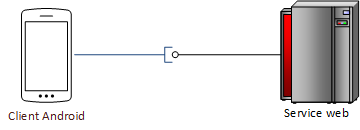
\includegraphics[width=\linewidth, height=\textheight, keepaspectratio]{archi_finale.png}
        \caption{Architecture proposée}
        \end{figure}
      \end{column}
    \end{columns}

    Objectif : utiliser simplement un service web.
    Architecture en 2 parties :
    Service Web : gestion des données
    Un client mobile : demande et fournit les données
    Communication du client avec le service. Le client ne sait “rien faire” dans un premier temps. Il délègue tout au service (stockage, traitement des données).
    Répartition des tâches :
    Client : Benoît
    Service : Benjamin
    Echange de rôles pour avoir le point de vue de chacun -> pas possible car mettre en place une solution de base a pris du temps et il a fallu apporter des améliorations
  \end{frame}

  \subsection{Spécifications}
  \begin{frame}{\subsecname}
    Serveur :
    REST
    Traite des requêtes clients et y réponds
    Stockage des données
    Fonctionnalités minimales :
    Connexion / Déconnexion du service
    Fournir la liste des personnes connectées
    Récupérer la position  d’un utilisateur
    Fournir les positions des utilisateurs
    Possibles améliorations :
    Historique de positions
    Calcul d’itinéraires
    Partage de position (sms, mail, etc)
  \end{frame}

  \begin{frame}{\subsecname}
    Android :
    Un client
    Le fonctionnement dépend du serveur
    Mobile
      Avoir la carte sur soi
      Volonté d'effectuer du développement mobile
    But
      Servir d'interface aux utilisateurs finaux

    Doit :
    Gerer un utilisateur
    Rendre le service de localisation
    Consommer le service web
    Répondre à des critères minimaux
      utilisabilité
      performances

    Pourra:
    Visualisation dans une carte 3D
    Visualisation en réalité virtuelle
    Ajout d'informations personnalisées
  \end{frame}


  \section{Réalisation de la solution}
  \subsection{Technologies transverses}
  \begin{frame}{\subsecname}
    Intégrations continue :
    TravisCI
    Tests automatiques, non régression
    Builds automatiques
    Déploiements automatiques
    Éviter les tâches répétitives et les erreurs
    Gestion du code source :
    GitHub
    Issues pour discuter des fonctionnalités et problèmes
    Itérations pour avoir des objectifs dans le temps
    Project pour définir les tâches  
  \end{frame}

  \subsection{Technologies mobile}
  \begin{frame}{\subsecname}
    Technologies
    Android
    Système
    Framework (>12)
    Android Studio

    Gestion du réseau
    Volley
    Picasso
    Bibliothèque graphique
    OpenGL ES
  \end{frame}

  \subsection{Réalisation mobile}
  \begin{frame}{\subsecname}
    Principe MVC

    3 activités
    = unité d’action
    Des fragments

    Utilisation de services asynchrones
    Communication réseau
  \end{frame}

  \subsection{Technologies serveur}
  \begin{frame}{\subsecname}
    Technos - Serveur
    Framework NodeJS, avec plusieurs paquets (npm) :
    Express : serveur web
    Jasmine : tests par specs
    MongoDB : Base de données
    Winston : Logs
    Fonctionnalités ajoutées :
    DNS
    Https
    DynDNS
    Logs d’erreurs / débug
  \end{frame}

  \subsection{Réalisation serveur}
  \begin{frame}{\subsecname}
    Réalisation Server (archi + explications + process mis en place)
    Utilisations :
    Requêtes : server.js, Express
    Données : database.js , MongoDB wrappé par service.methods.js
  \end{frame}

  \section{Résultats}
  \subsection{Service à disposition}
  \begin{frame}{\subsecname}
    Plusieurs URLs:
    /GET
    Who : liste des personnes connectées
    Where : positions des personnes connectées et informations supplémentaires
    /POST
    Login : se connecter
    Logout : se déconnecter
    Where : mettre à jour sa position
    Exemple de paramètres pour une requête (/POST where){
        "token": "1A2Z3E4R5T6Y7U8I9O0P",
        "location": [
            1.0,
            2.0,
            3.0
        ]
    }  
  \end{frame}

  \subsection{Client Android}
  \begin{frame}{\subsecname}
    Un client potentiel du service.

    Localisation
    Affichage des utilisateurs connectés
    Synchronisation de la position avec le serveur
    Définition de points d’intérêt
    Affichage 3D

    Communication
    Authentification Google
    Partage de position
    22

    Fonctionnement
    Authentification
    Parcours de la carte
    Navigation dans le menu
    
  \end{frame}

  \subsection{Améliorations possibles}
  \begin{frame}{\subsecname}
    Client
      Amélioration de l’interface du client
      Mode réalité virtuelle
        Google cardboard
      Gestion des étages
        Calibration

    Serveur
      Calcul d’itinéraires
      Gestion des logs, alertes automatiques (erreurs graves)
    
  \end{frame}
  
%---------- Conclusion

  \section{Conclusion}
  \begin{frame}{\secname}
      \begin{block}{Rappels}
        \begin{itemize}
          \item Suivi de personnes
          \item Service web : réceptionner et traiter des données
          \item Client : fournir et demander des données
        \end{itemize}
      \end{block}

      \pause

      \begin{alertblock}{Points négatifs}
        \begin{itemize}
          \item Client uniquement android : iOs, Windows Universal, Site web
          \item Déploiement sur le cloud
        \end{itemize}
      \end{alertblock}

  \end{frame}

  \begin{frame}{\secname}
    \begin{exampleblock}{Points positifs}
        \begin{itemize}
          \item Architecture modulaire
          \item Processus d'intégration
          \begin{itemize}
            \item Intégration continue
            \item Tests automatiques
            \item Déploiement automatique
          \end{itemize}
        \end{itemize}
      \end{exampleblock}

      \pause

      \begin{block}{Perspectives}
        \begin{itemize}
          \item Projet accessible librement sur GitHub
          \item Tout le mode peut y contribuer
        \end{itemize}
      \end{block}
  \end{frame}

%---------- Remerciement

  \begin{frame}{Fin}
    \begin{center}
      Merci de votre attention.
    \end{center}
  \end{frame}

\end{document} %finished!
